\documentclass[border=10pt]{standalone}
%%%<
\usepackage{verbatim}
%%%>
\usepackage{pgfplots}
\pgfplotsset{width=7cm,compat=1.8}
\begin{comment}
:Title: Stacked bar plot
:Tags: 2D;Stacked plots;Manual
:Author: Christian Feuersänger
:Slug: stacked-bar-plot

Stacking plots means to add either x or y coordinates of
successive \addplot commands on top of each other.

The code is from the PGFPlots 1.10 manual: "4.5.8 Stacked Plots",
"Stacked Bar Plots and Nodes Near Coords".
\end{comment}
\begin{document}
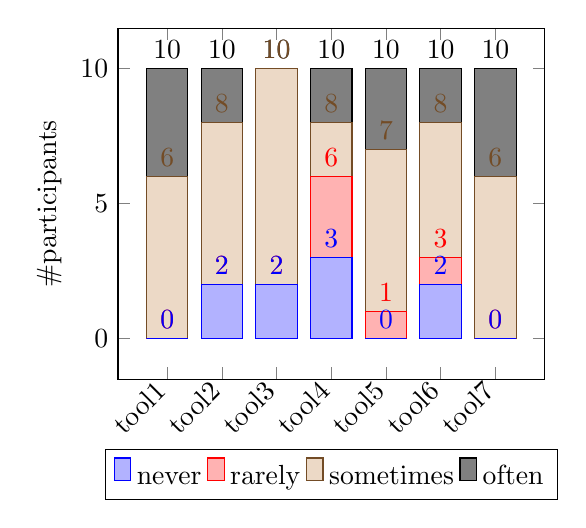
\begin{tikzpicture}
\begin{axis}[
    ybar stacked,
	bar width=15pt,
	nodes near coords,
    enlargelimits=0.15,
    legend style={at={(0.5,-0.20)},
      anchor=north,legend columns=-1},
    ylabel={\#participants},
    symbolic x coords={tool1, tool2, tool3, tool4, 
		tool5, tool6, tool7},
    xtick=data,
    x tick label style={rotate=45,anchor=east},
    ]
\addplot+[ybar] plot coordinates {(tool1,0) (tool2,2) 
  (tool3,2) (tool4,3) (tool5,0) (tool6,2) (tool7,0)};
\addplot+[ybar] plot coordinates {(tool1,0) (tool2,0) 
  (tool3,0) (tool4,3) (tool5,1) (tool6,1) (tool7,0)};
\addplot+[ybar] plot coordinates {(tool1,6) (tool2,6)
  (tool3,8) (tool4,2) (tool5,6) (tool6,5) (tool7,6)};
\addplot+[ybar] plot coordinates {(tool1,4) (tool2,2) 
  (tool3,0) (tool4,2) (tool5,3) (tool6,2) (tool7,4)};
\legend{\strut never, \strut rarely, \strut sometimes, \strut often}
\end{axis}
\end{tikzpicture}
\end{document}
